\chapter{DLT and IoT in Business}
This chapter aims to provide a brief background on Distributed Ledger Technology and Internet of Things in industry and confidently present a few use cases to bridge both worlds.\acrfull{dlt}, private, permissioned or consortium blockchains are used interchangeably in this chapter. 

\section{Distributed Ledger Technologies} 
As discussed in chapter 2, a blockchain is essentially a trustless, \acrshort{p2p}, append-only list of records verified and shared among participants in the network. With the rise of Ethereum, blockchains gained Turing completeness and an easier way to implement business logic and automate procedures, called smart contracts. As seen from Bitcoin and Ethereum, those kind of networks tend to be slow and too expensive to maintain due to their public nature. Private and consortium blockchains could benefit from stripping down some mechanisms and thus a new design emerged for business and enterprise environments where all participants are known, cutting down unnecessary overheads and architectural choices used in permissionless or public blockchains. 

As Vitalik Buterin defined consortium blockchains in \cite{buterin2015public}:
\begin{quote}
    \textit{A consortium blockchain is a blockchain where the consensus process is controlled by a pre-selected set of nodes; for example, one might imagine a consortium of 15 financial institutions, each of which operates a node and of which 10 must sign every block in order for the block to be valid. The right to read the blockchain may be public, or restricted to the participants, and there are also hybrid routes such as the root hashes of the blocks being public together with an API that allows members of the public to make a limited number of queries and get back cryptographic proofs of some parts of the blockchain state. These blockchains may be considered ``partially decentralized".}
\end{quote}

In the upcoming subsections we discuss how consortium blockchains differ from permissionless on each of their attribute and why they can still work. The main criteria for designing such networks are incentive compatibility, responsiveness and finality of transactions. We follow the structure of comparison of this work \cite{dib2018consortium}.   

We should state that blockchains, especially in Europe, need to be designed in such a way that respect users' data privacy under the European General Data Protection Regulation. Consortium blockchains need to be compliant with such regulations \cite{gdpr}.

\subsection{Immutability}
Immutability in permissionless blockchains comes from energy expenditure of Proof of Work and from the protocol that each node builds and propagates the longest chain.

In consortium blockchains, since validator nodes are under known parties it could be infeasible for the majority to agree and change the history of the chain. Could be done but only if everyone agrees. Also a hash could be periodically published on permissionless chain in order to know what the current state of the consortium chain was. Recomputing the hashes would be trivial without \gls{pow}. However if members can come to an agreement, they could alter the history of the blockchain, since such actions are considered controversial and go against the immutability aspects of blockchains, a major selling point, a periodic public hash would suffice to let everyone know that history has been modified. As we mentioned earlier there might be a good reason to modify a chain, and that is due to regulations. Since members are known they can be fined by governments and even shut them down if they do not comply. In a permissionless network that would be impossible.

\subsection{Access and Privacy}
A blockchain is based on a \acrshort{p2p} network that propagates transactions and new blocks, fundamentally linking its members. Each new node on the network is connected to a neighbor and start receiving blocks, in the meantime it validates each block and cross references it with other neighbors.  In figure \ref{fig:btc-nodes} we see the distribution of bitcoin nodes in Europe. Each user uses their private key to derive their address, which is their public identity and uses a node to transact with a network. Users might run their own full nodes or use third party services and light nodes. 

\begin{figure}[h]
    \centering
    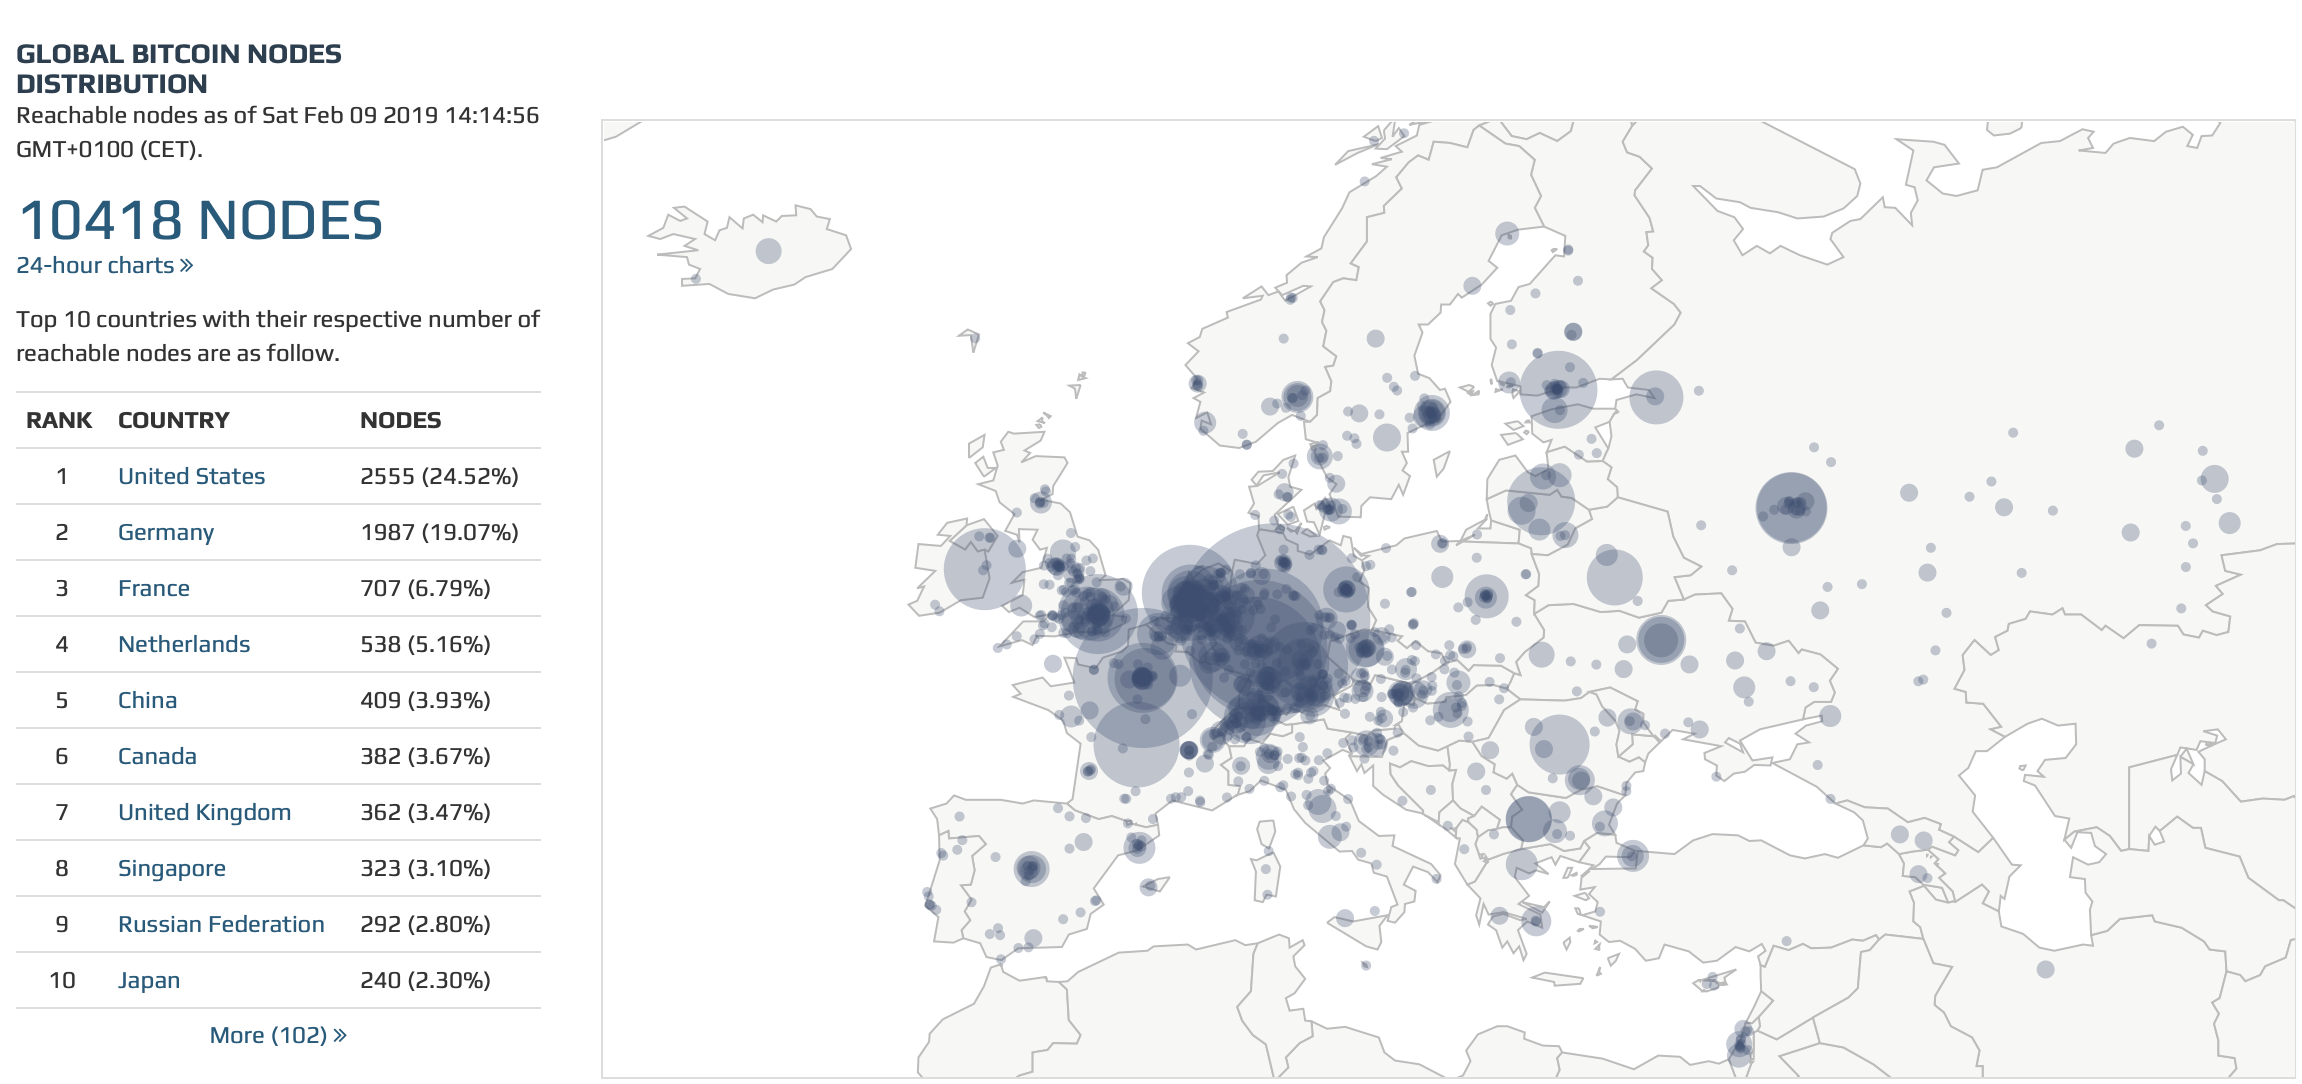
\includegraphics[width=1\textwidth]{images/BTCnodes.png}
    \caption{Bitcoin nodes distribution in Europe \cite{bitnodes}}
    \label{fig:btc-nodes}
\end{figure}

In the consortium setup each user is identified by its node and its certificate that is registered with a \acrfull{msp}. More details on how that works on \ref{ch:Fabric} where we dive in our consortium blockchain of choice, Fabric. Participant nodes build the ledger from the genesis block. When a new member joins the network, depending on the use case, previous blocks could be gained through a similar \acrshort{p2p} approach. We should state that this restricted setup ensures data privacy by default. Encrypting transactions is not easily doable since they are needed to verify the previous blocks. There is a solution with zero knowledge proofs that allows for the authentication of transactions without giving away any personal information of either the sender or receiver\cite{reitwiessner2016zksnarks}.

\subsection{Mining, consensus and incentive compatibility} 
On of the most important aspects of a blockchain network is how it reaches finality and how it incentivizes its participants to play along. Permissionless and Permissioned networks are based on a whole two different approaches. One is based on cryptocurrency economics\cite{schrijvers2016incentive}, where the currency is a crucial attribute of the network whereas the other is based on reputation and lawsuits.

As we have previously stated, miners are nodes that are sharing, or collaborating with a mining pool, their computational power in order to solve the \gls{pow}. Their reward on Bitcoin and Ethereum are some BTC or ETH per block, specifically as of February 2019, 12.5BTC and 3ETH per block. Each transaction has a fee paid to the miners for their expenditures on hardware and electricity and also to incentivize them to include their transactions in the next block. This protocol and game, secures the network against 51\% attacks. That means that an adversary can rewrite the history only if it holds the 51\% of the network's hashing power, but that on most occasions is counter-incentivized, the gains would be lower that what he spends. Practically as low as 33\% for a double spend attack \cite{eyal2018majority}.

On the contrary, in consortium blockchains validating nodes can be trusted in some degree and everything about their identity is known. In these setups, consensus can be simplified and there is no need for such secure and energy wasteful mechanisms as \gls{pow}. Security and trust comes from the permissioned network which is, by definition, Sybil proof, something that public blockchains need to mitigate\cite{dionyziz-sybil} \cite{mitigate-sybil}.

\subsection{Forks, responsiveness and finality of transactions}
In permissionless chains, blocks are added to the chain with an interval, commonly ranging between some seconds for Ethereum and a few minutes for Bitcoin (on an average, 15 seconds and 10 minutes respectively). Finality of a transaction comes after some time where the probability of a number of blocks to appear and make the current chain the longest is negligible. For bitcoin we wait for six confirmations, or six blocks (1 hour) and only then we consider a transaction as finalized. This is all done due to forks, where the longest chain is accepted on the network. That means if someone could compute blocks given a point in the past and continue their version of the chain, if they succeed in making a heavier chain then this will be the new chain. 

In figure \ref{fig:longest-chain}, we have an orphan block\footnote{An orphan block, in the context of Bitcoin, is a valid block that was computed but not accepted by the network because another valid block referencing the previous arrived first.}(purple), the main chain (blue) that everyone uses and a secret, unpublished chain (red). The secret chain is longer than the main chain and has the potential, when published, to be accepted by everyone, thus having the capacity to revert old transactions\footnote{Letters within the blocks denote a different set of transactions.}.  
\begin{figure}[h]
    \centering
    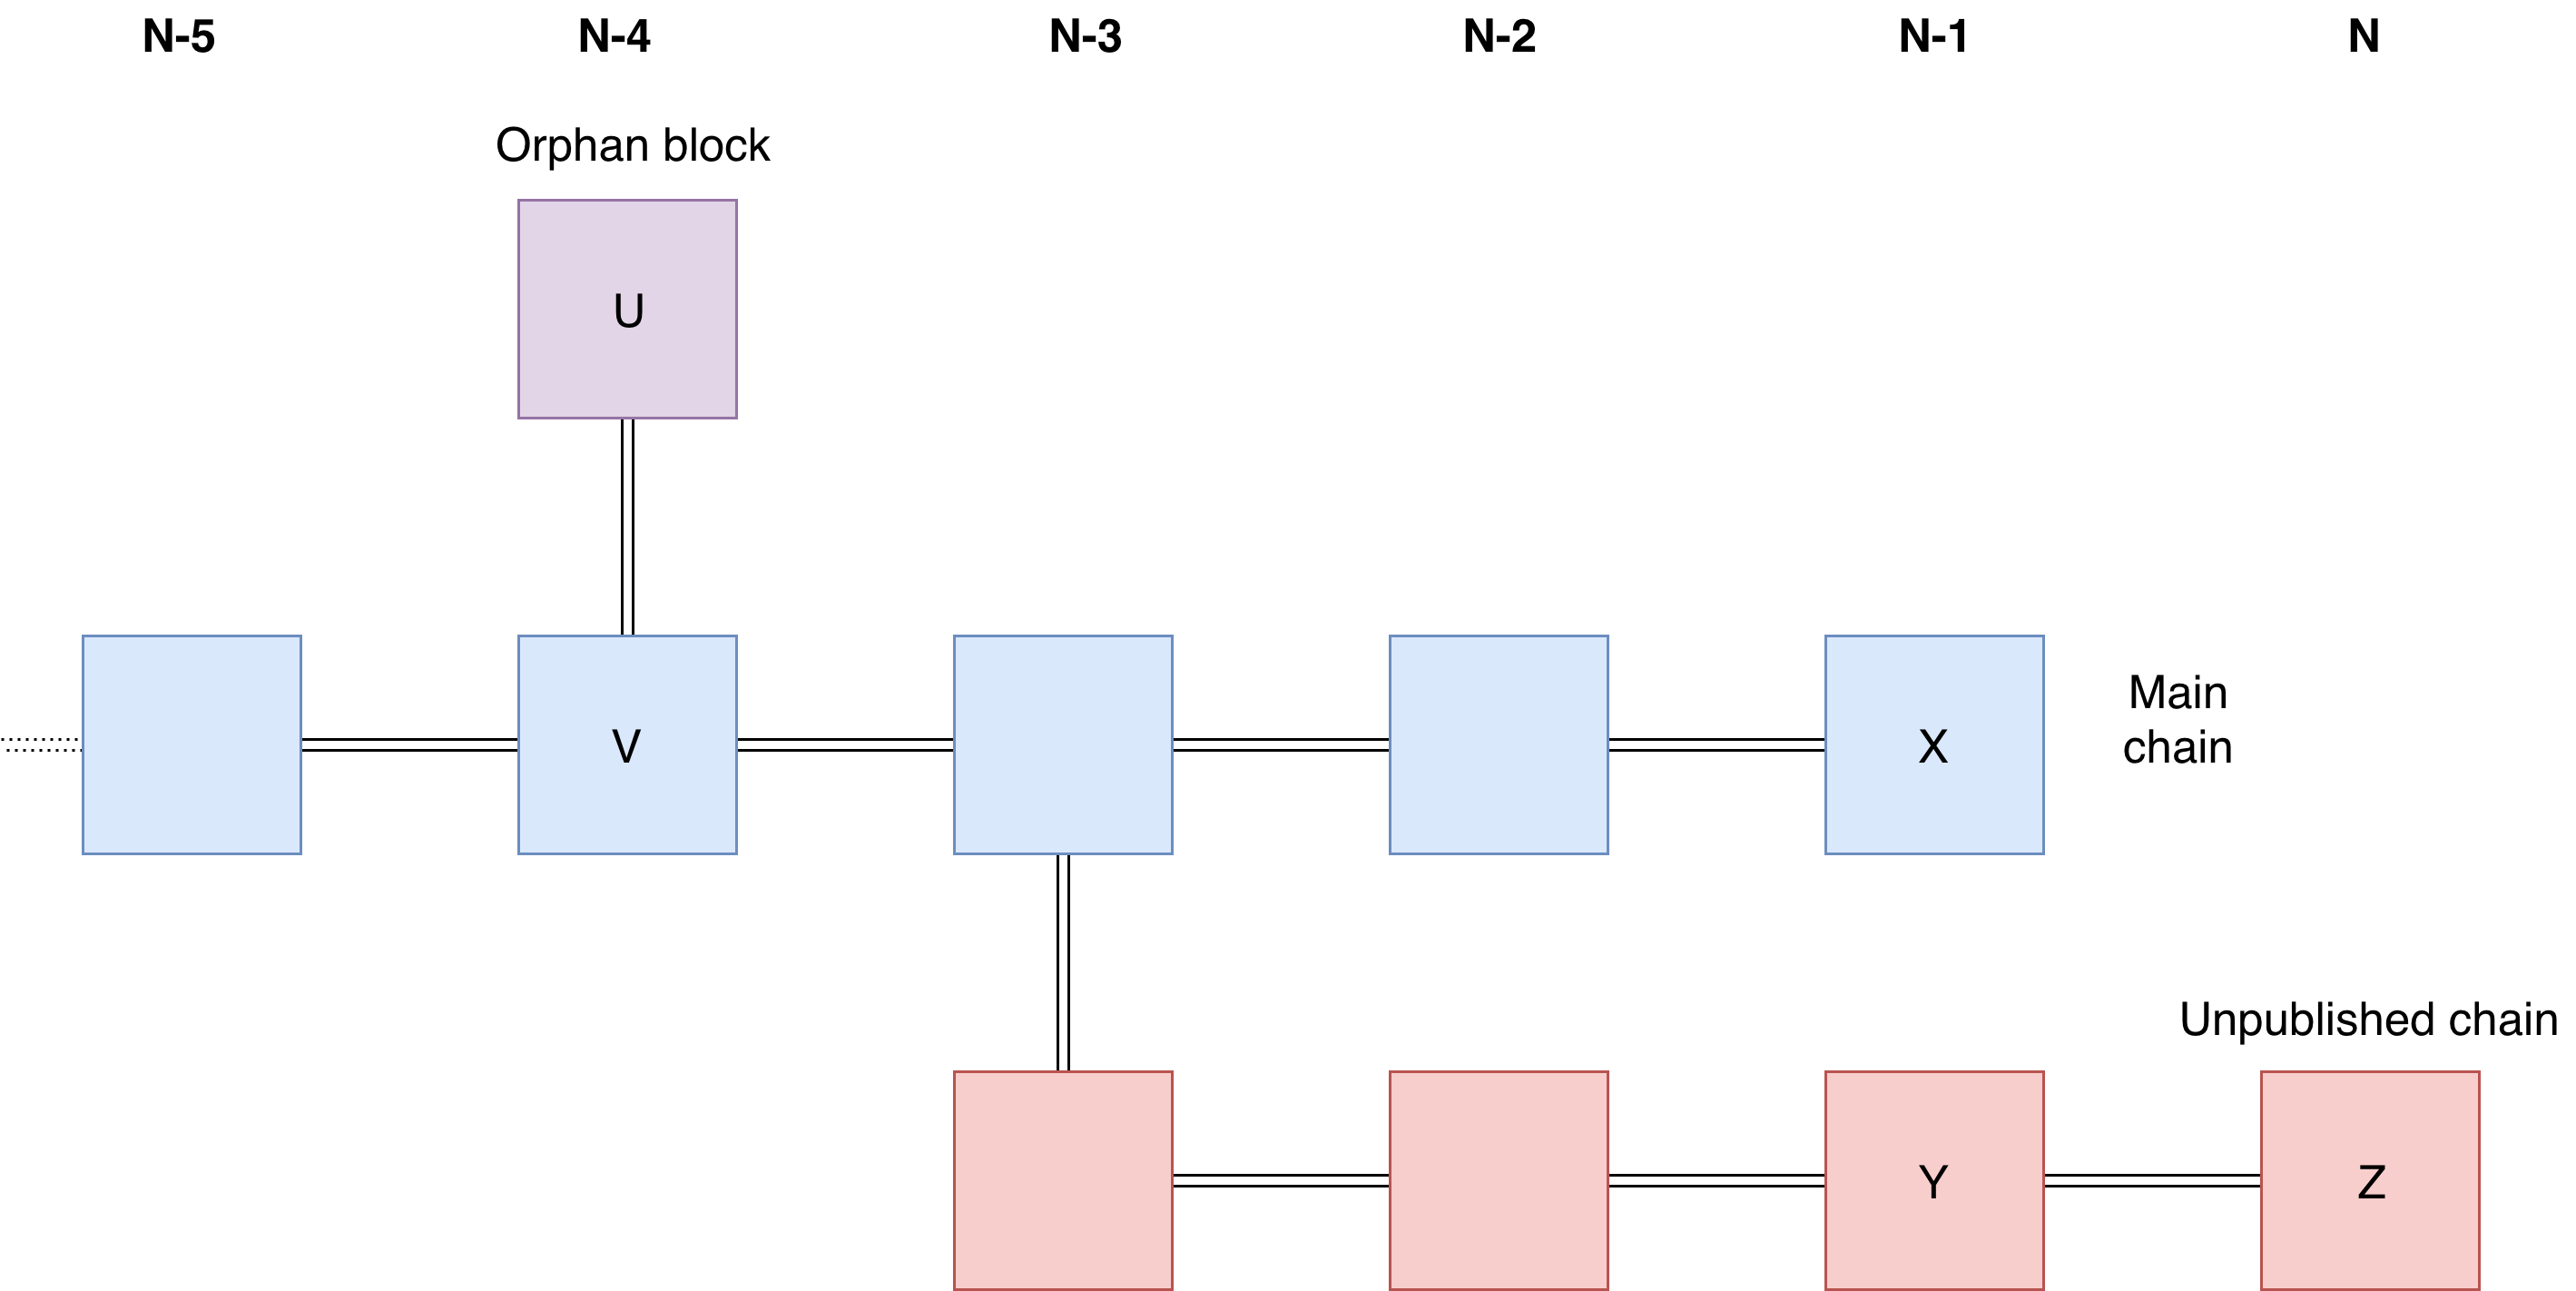
\includegraphics[width=1\textwidth]{images/forks.png}
    \caption{A new longest chain (red) reverts transactions on main chain (blue).}
    \label{fig:longest-chain}
\end{figure}

On the other hand, in consortium blockchains, we do not have a risk of a new set of blocks appearing and making the old chain obsolete, every transaction upon ordering is considered as final. In addition, we do not need a block interval as well as to wait for confirmations, or new blocks on top of the associated transaction, thus making the network a lot more responsive. Blocks are created on demand and everyone works on the main chain. We could say that when participants are known, everything is more predictable and linear.

% One more important aspect that falls under this category is that in consortium blockchains 
% is the easiness of upgrading the protocol. The peers in the network get upgraded d Contradictory to "soft" and "hard forks" needed on permissionless chains where  (transaction backward compatibility).

% One more important benefit of having a consortium chain is the easiness of upgrading the protocol. Contradictory to upgrading the protocol on a permissionless network where disruption in the network might occur. 

\subsection{Smart Contracts}
Bitcoin offers very strict functionality for security, while Ethereum offers Turing completeness, it is rarely used due to undecidability \cite{miller-turing}. Contracts in order to pass security audits needs to be deterministic and every state easily analyzed. 

In consortium blockchains we can have more complex functionality that does cost orders of magnitude less to operate and it is easily scalable, since  smart contracts do not need to be executed on every single node but only on nodes that have them installed and are instructed to run them. In this way we achieve greater level of parallelazation and scalability.

To conclude this section, due to the known participants on a consortium network it is possible to strip some expensive mechanisms that offer security and stability in permissionless networks, simply because they are not needed. By adapting the permissioned networks, we achieve higher throughput, greater responsiveness and flexibility. 